\section{Conclusion}

\begin{frame}
	\frametitle{\insertsectionhead}
	\begin{block}{Module actuel : support de }
		\begin{itemize}
			\item lecture / écriture
			\item SHA256
			\item AES-XTS, AES-CBC
			\item plain et plain64
		\end{itemize}
	\end{block}
	\pause
	\begin{block}{Suite du projet}
		\begin{itemize}
			\item amélioration du code
			\item scripts de tests
			\item revue par les développeurs FreeBSD
			\item ajout de fonctionnalités
		\end{itemize}
	\end{block}
\end{frame}

\begin{frame}
	\centering
	Questions ?
\end{frame}

\begin{frame}
	\begin{figure}
		\frametitle{Démarrage}
		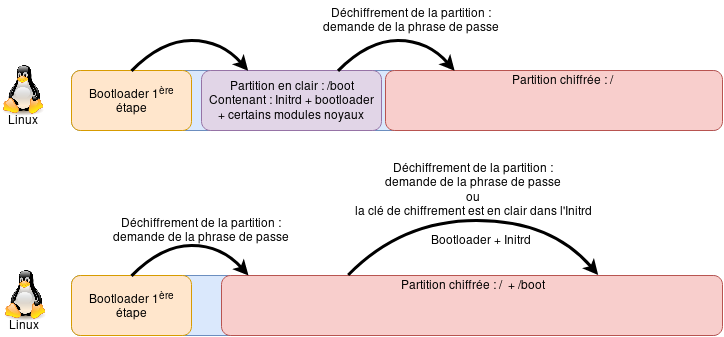
\includegraphics[width=.9\textwidth]{conclusion/DemarrageLinux}
		\caption{Démarrage sous Linux}
	\end{figure}
\end{frame}

\begin{frame}
	\begin{figure}
		\frametitle{Démarrage}
		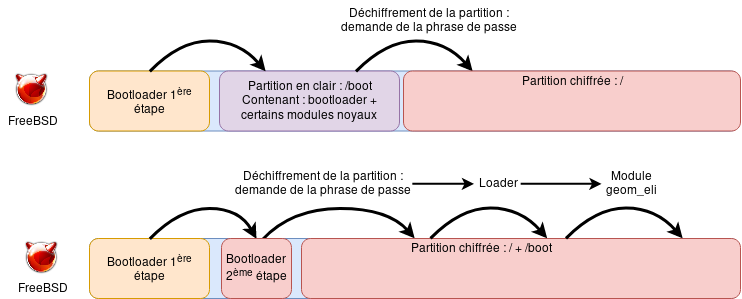
\includegraphics[width=.9\textwidth]{conclusion/DemarrageFreeBSD}
		\caption{Démarrage sous FreeBSD}
	\end{figure}
\end{frame}
